\chapter{FX}

Odin 2 comes with four internal FX modules: \fat{Delay, Chorus, Phaser} and \fat{Flanger}.

\begin{center}
    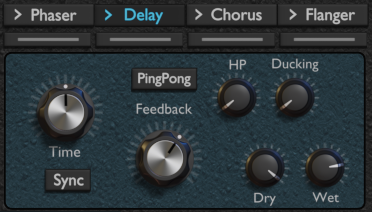
\includegraphics[width=0.4\textwidth]{graphics/FX.png}
\end{center}

The buttons on top of the FX modules serve multiple purposes:

\begin{center}
    
\includegraphics[width=0.4\textwidth]{graphics/FX_selector.png}
\end{center}

Clicking the corresponding name of the module reveals the corresponding module. The buttons below the module name are used to turn enable or disable the module.
You can also \fat{change the order of the modules}, by drag'n'dropping their name handles to the left or right.

\audioparameter{FX On}{0}{1}{
    Use the buttons below the module name to turn the FX module on or off. All modules can be used at the same time.
}

\audioparameter{FX Order}{0}{0}{
    Drag'n'drop the FX module handles to change the order of the FX. The algorithms are calculated in series from left to right.
}

\section{Delay}
\label{delay}

A delay is a module capable of producing an 'echo' effect: The signal is fed into a delay-line, which outputs the signal again after a set amount of time again. The output of the delay line can also be fed back in, allowing a chain of attenuating echos. By controlling the delay time and feeback parameters, a wide variety of effects can be achieved. The Delay module in Odin 2 goes a step further and offers several additional features.

\audioparameter{Delay Time}{1}{1}{
    Controls the time the delay line takes to output the sound again. Depending on the parameter "Delay Sync", this is either a dial for continuous values in Hz, or a custom selector to sync the time to the beat. This selector allows for arbitrary fractions of the current host BPM, for example 5/16th notes:

    \begin{center}
        
\includegraphics[width=0.18\textwidth]{graphics/delay_sync.png}
    \end{center}
}

\audioparameter{Delay Feedback}{1}{1}{
    Controls how much of the output of the delay line is fed back in again. If feedback is zero, only one echo will be audible. If feedback is one, an infinite series of exact copies of sound will be output. Everything inbetween makes for slowly attenuating echos.
}

\audioparameter{Delay Sync}{0}{1}{
    Controls whether the Delay Time is set by a knob in Hz or via the sync-time selector, syncing it to the host BPM.
}

\audioparameter{Delay PingPong}{0}{1}{
    Enabling PingPong will make the left and right stereo delay lines crossfeed: The output of the left line is fed into the right line and vice versa.

    The initial input into the delay lines is mixed down to a mono signal and then fed into the left delay line only. The dry signal remains in the center of the stereo field.
}

\audioparameter{Delay Highpass (HP)}{1}{1}{
    The processed signal in the Delay module is filtered through a 6dB/Oct highpass filter. The Delay Highpass parameter controls the cutoff of this internal filter. This is great for removing the muddiness that deep frequencies can produce in a delay module.

    Note that the highpass filter is not applied inside, but after the feedback loop, i.e. consecutive echos do not get filtered further more as they are processed again.
}

\audioparameter{Ducking}{0}{1}{
    Ducking attenuates the output of the delayed signal if an input signal is present. This is great for decluttering sections where the delayed signal interferes with the unprocessed signal.
}

Unlike the other FX modules, the Delay features a separate Dry and Wet control to allow for easier adjustments of processed and unprocessed signals individually.
\audioparameter{Delay Dry}{1}{1}{
    Controls how much unprocessed signal is output by the Delay.
}

\audioparameter{Delay Wet}{1}{1}{
    Controls how much processed signal is output by the Delay.
}